\chapter{Solução proposta\label{cap:desenvolvimento}}

\section{Introdução}

Neste capítulo é apresentada a solução proposta para controle de acesso físico utilizando tecnologia de biometria e uma aplicação web. Essa solução trata-se de um sistema eletrônico baseado em \textit{hardware} e \textit{software} livre. Tal sistema utiliza a impressão digital como característica biométrica para a autenticação de usuários. A autenticação de impressões digitais é um processo de segurança utilizado em ambientes que necessitam do controle de entrada de pessoas, a fim de restringir o acesso às pessoas autorizadas. O sistema em questão é batizado de Setfinger. Esse sistema é composto por dois elementos: um cliente e um servidor. O cliente é o aparelho responsável pela interface com o usuário, leitura de impressões digitais e controle de fechadura eletrônica (fecho elétrico). O servidor propriamente dito, aqui chamado de Setserver, é a máquina na qual devem ser instalados os serviços de conexão TCP, banco de dados e plataforma web. Portanto, o Setserver é composto por um servidor TCP baseado em node.js, um banco de dados Mysql e uma plataforma de gerenciamento web. O servidor TCP é responsável por criar uma conexão do tipo TCP, manter a comunicação com o cliente e gravar informações no banco de dados, de acordo com os comandos enviados pelo cliente. O banco de dados armazena os cadastros e os registro de acesso dos usuários. Por fim, a página web provê o gerenciamento dos dados mantidos no banco de dados, tais como, atualização e exclusão de cadastros, consulta da frequência de usuários, em tabelas ou gráficos, e a obtenção de relatórios. O cliente e o servidor se comunicam via conexão TCP/IP, em uma rede de computador, como ilustrado na Figura~\ref{rede_setfinger}. A seguir, são apresentados os objetivos do sistema Setfinger.

\begin{figure}[!ht]
  \begin{center}
  \caption{Sistema Setfinger instalado em uma rede local - Exemplificação de comunicação entre o aparelho Setfinger (cliente) e o servidor, através de uma Rede local.}
  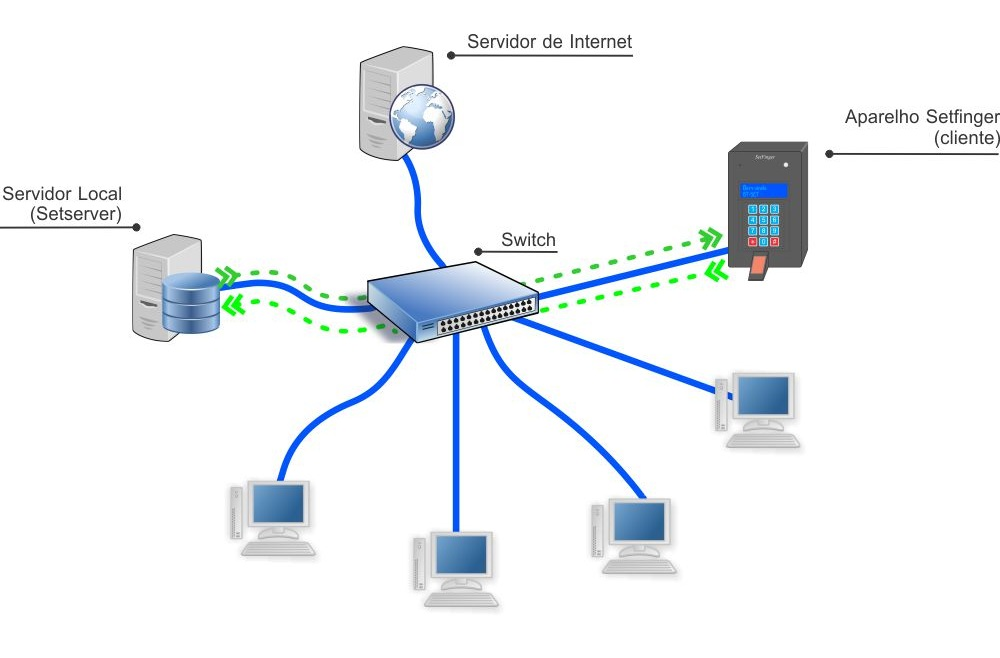
\includegraphics[scale=0.6]{figuras/cap4/rede_setfinger.jpg}\\
  Fonte: Elaborada pelo autor.
  \label{rede_setfinger}
  \end{center}
  \end{figure}

\section{Objetivos do sistema Setfinger\label{objetivos_sf}}

O sistema Setfinger foi desenvolvido no Grupo Servidor de Estação de Trabalho (GT-SET) do Centro de Tecnologia da Informação e Comunicação (CTIC) da Universidade Federal do Pará (UFPA). Essa solução foi elaborada com o propósito de atender as demandas de controle de acesso físico interno da UFPA. Os principais objetivos definidos na elaboração do projeto Setfinger são:

\nomenclature{GT-SET}{Grupo Servidor de Estação de Trabalho}
\nomenclature{CTIC}{Centro de Tecnologia da Informação e Comunicação}



\begin{itemize}

\item Substituir o uso de chaves por biometria

O espaço interno do CTIC é dividido em salas, porém o acesso ao prédio é livre para atendimento ao público. Desta forma, a porta de cada sala deveria permanecer trancada para evitar que visitantes tenham acesso direto a elas. No entanto, a utilização de chaves para trancar e destrancar a porta repetidas vezes, pode se tornar um processo incômodo para os usuários. Sendo assim, a utilização de tecnologia biométrica torna-se um processo mais rápido e prático, uma vez que não há a possibilidade do usuário esquecer ou perder a chave de acesso (biometria). 


\item Aumentar a segurança de usuários e bens

Garantindo a restrição de acesso para usuários não autorizados, pode-se proporcionar maior segurança para os usuários e evitar possíveis incidentes envolvendo pessoas não integrantes às salas.


\item Registrar o acesso de bolsistas e servidores para controle de ponto

O uso de um sistema digital torna mais eficiente o registro de acesso de pessoas em um determinado local. Isso automatiza o processo de controle de ponto, garante maior segurança às informações registradas e torna os dados mais acessíveis para supervisores e supervisionados.  


\item Gerar relatório de acesso

Através dos registros de acesso dos usuários, pode-se gerar relatório para avaliação ou comprovação de frequência.


\item Redução de custos

Na porta de entrada principal do CTIC é utilizado um dispositivo de controle de acesso semelhante ao modelo F7, apresentado na Seção~\ref{F7}. O objetivo do CTIC é que cada sala disponha de um aparelho de controle de acesso biométrico. O ideal seria que, além do CTIC, outros espaços da UFPA contassem com esse tipo de controle, porém esse dispositivo foi adquirido pelo valor de R\$ $2.400,00$ (dois mil e quatrocentos reais). Esse valor representa um custo alto para a UFPA. Desta forma, há a necessidade de uma solução de custo reduzido, em relação as soluções de mercado, e com licença livre para que o próprio usuário (administrador) possa fazer a manutenção do sistema.

\end{itemize}

\section{Hardware}

O principal dispositivo utilizado no conjunto de \textit{hardware} do sistema Setfinger é o Arduino Mega, uma ferramenta de prototipagem eletrônica \textit{open-source} que tem sido amplamente utilizada no ambiente acadêmico para o desenvolvimento do conhecimento de eletrônica, \textit{hardware} e sistemas embarcados. Essa plataforma permite o desenvolvimento de soluções para inúmeros tipos de aplicações e problemas, podendo ser integrado a sensores e outros componentes que ampliam sua capacidade de interação. Em comparação a outras opções de \textit{hardware} microcontrolado, o Arduino é um dos mais populares, possui grande oferta no mercado, tem custo relativamente baixo e programação de alto nível. Além disso, a comunidade do Arduino é composta por um número grande de desenvolvedores, fóruns de discussões e materiais que facilitam o uso da placa para a elaboração de projetos simples ou complexos. Esses foram os principais aspectos que motivaram a escolha do Arduino para a elaboração do módulo de \textit{hardware} aqui proposto. Além disso, o ambiente de desenvolvimento em que a solução proposta é projetada pratica uma política de criação de soluções baseadas na filosofia \textit{open source}. Por isso, o principal critério avaliado na escolha dos recursos utilizados na execução deste projeto é a licença \textit{open-source}. Além do Arduino, são utilizados componentes selecionados de acordo com a sua popularidade, compatibilidade com o microcontrolador, suporte, custo e oferta no mercado, pois alguns componentes são escassos no mercado brasileiro, possuem preços elevados e não apresentam documentação. Portanto, nesta seção é apresentado o \textit{hardware} do aparelho Setfinger proposto, bem como o material e as técnicas utilizadas no seu desenvolvimento, e o papel de cada um dos elementos que o compõem.


\subsection{\textit{Hardware} Setfinger proposto \label{hardware_setfingerproposto}}

De acordo com os objetivos definidos na Seção~\ref{objetivos_sf}, é proposto um aparelho biométrico com \textit{hardware} baseado em plataforma Arduino. Tal aparelho é dividido em dois módulos: um módulo de interface com o usuário e um módulo de \textit{hardware} interno (veja a Figura~\ref{setfinger_modulos}). O módulo de interface com o usuário permite a interação do usuário com o sistema Setfinger. Esse módulo é composto por um display LCD, um teclado matricial e um leitor de impressões digitais. O módulo interno é composto por um Arduino Mega 2560, um ethernet shield W5100 e uma placa de integração de componentes, denominada Setshield, a qual é responsável por conectar ao Arduino os componentes apresentados na Tabela~\ref{tabela_componentes}. A placa Setshield presente no módulo de \textit{hardware} interno, contém um relé que deve ser associado em série ao fecho elétrico que controlará a abertura da porta que dá acesso ao ambiente a ser controlado. Portanto, é necessária a divisão do aparelho em dois módulos para evitar, em casos de arrombamento do aparelho, que usuários mal intencionados tenham acesso a esse relé.

Além do \textit{hardware} proposto aqui, são apresentadas outras duas versões de \textit{hardware} no Apêndice~\ref{hardware_1.0} e Apêndice~\ref{hardware_2.0}. No entanto, a versão proposta apresenta um projeto de \textit{hardware} otimizado, em relação as demais versões, pois nessa versão de \textit{hardware} o circuito da placa Setshield apresenta um layout menor e há uma redução na quantidade de fios necessários para conectar os componentes ao Arduino.

Na Figura~\ref{diagrama_hardware}, é apresentado o diagrama de blocos que representa o layout do \textit{hardware} do Setfinger proposto. A partir desse diagrama é possível identificar todos os componentes de \textit{hardware} que integram o sistema Setfinger, e compreender a relação entre eles.

\begin{figure}[!t]
  \begin{center}
  \caption{Aparelho Setfinger - à esquerda da imagem é mostrado o módulo de interface com o usuário e à direita da imagem é mostrado o módulo de \textit{hardware} que deve ser instalado fora do alcance do usuário, de preferência no interior da sala a ser controlada. O módulo de \textit{hardware} interno é mostrado sem nenhuma proteção (carcaça), mas deve ser embutido em um gabinete plástico.}
  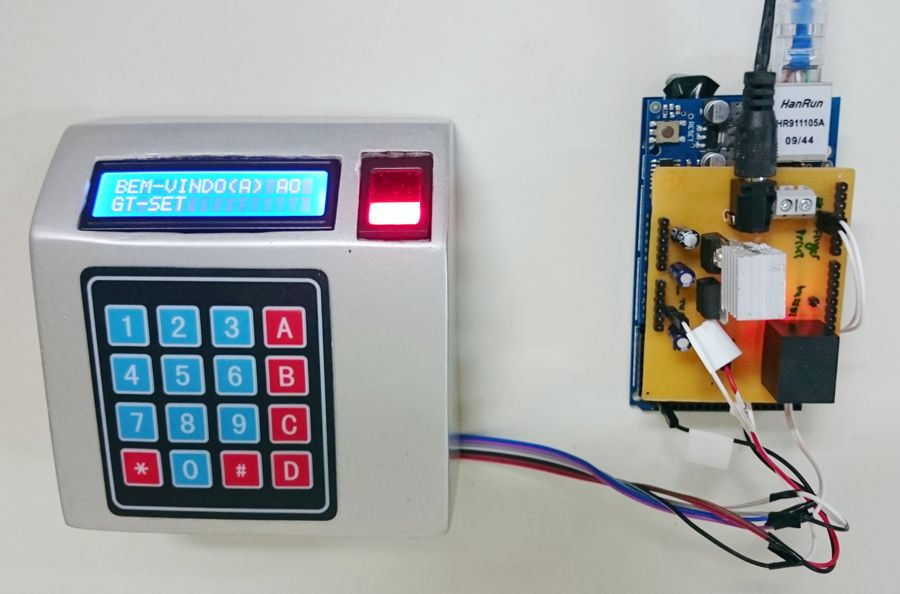
\includegraphics[scale=0.4]{figuras/cap4/setfinger_modulos.jpg}\\
  Fonte: Elaborada pelo autor.
  \label{setfinger_modulos}
  \end{center}
  \end{figure}
  
  
  
  
  \begin{table}[]
\centering
\caption{Tabela de componentes conectados ao Arduino através da placa Setshield.}
\label{tabela_componentes}
\begin{tabular}{ll}
\hline
%\multicolumn define as configurações de alinhamento e exibição de colunas
\multicolumn{1}{c}{\textbf{Quantidade}} & \multicolumn{1}{c}{\textbf{Componentes}} \\ \hline\hline
\multicolumn{1}{c}{1} & Relé CONT: $10$ A $125$ V AC/ COIL: $5$ V DC\\ \hline
\multicolumn{1}{c}{3} & Resistor $4.6$ k$\Omega$ \\ \hline
\multicolumn{1}{c}{3} & Resistor $1$ k$\Omega$\\ \hline
\multicolumn{1}{c}{2} & Capacitor $47 \mu$ F $16$ V\\ \hline
\multicolumn{1}{c}{1} & Capacitor $100 \mu$ F $16$ V\\ \hline
\multicolumn{1}{c}{1} & Regulador de tensão L7809\\ \hline
\multicolumn{1}{c}{1} & Regulador de tensão L7805\\ \hline
\multicolumn{1}{c}{1} & Conector Jack P4 para placa $2,1$ mm\\ \hline
\multicolumn{1}{c}{1} & Borne para placa (com parafuso)\\ \hline
\multicolumn{1}{c}{1} & Sensor Fingerprint ZFM-20\\ \hline
\multicolumn{1}{c}{1} & Display LCD 16x2 5V\\ \hline
\multicolumn{1}{c}{1} & Teclado matricial\\ \hline


\end{tabular}
\end{table}

  
  
  
\begin{figure}[!t]
  \begin{center}
  \caption{Diagrama de \textit{hardware} do aparelho Setfinger.}
  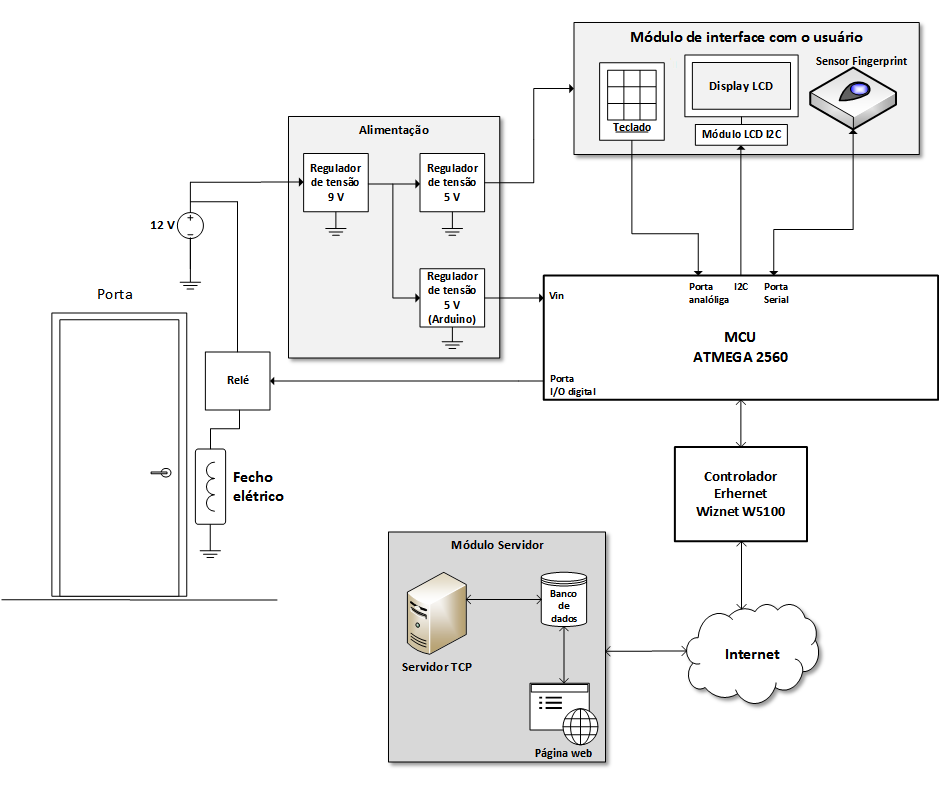
\includegraphics[scale=0.6]{figuras/cap4/diagrama_hardware.png}\\
  Fonte: Elaborada pelo autor.
  \label{diagrama_hardware}
  \end{center}
  \end{figure}
  
  
  
 A seguir, são descritas a atuação de cada elemento presente no diagrama de \textit{hardware} mostrado na Figura~\ref{diagrama_hardware}, assim como, suas características e funcionamento. Além disso, são apresentadas considerações importantes sobre a pinagem dos componentes, pois os barramentos de comunicação serial, como I2C, SPI, TTL, ou saídas digitais com sinal PWM, estão presentes em pinos específicos da Unidade de Microcontrolador (\textit{microcontroller unit} -- MCU). Portanto, a conexão de cada dispositivo deve ser realizada de acordo com o seu tipo de comunicação. Normalmente, a pinagem adequada para cada componente é informada pelo fabricante.
 
 \nomenclature{MCU}{Microcontroller Unit}
 
\begin{itemize}
    
    \item Fecho elétrico
    
    O fecho elétrico é um dispositivo instalado junto a fechadura da porta e pode ser controlado eletronicamente. Os fechos elétricos utilizados neste trabalho operam sob uma tensão de $12$ V. Esses dispositivos possuem um solenoide em seu interior. Ao ser energizado, o solenoide move uma pequena peça que destrava a fechadura e permite a abertura da porta. Alguns modelos de fecho elétrico possuem um mecanismo chamado de memória, com esse mecanismo basta que o solenoide seja energizado por um instante e a fechadura permanecerá destravada até que a porta seja aberta. Nos mecanismos sem memória, a fechadura só permanece destravada enquanto o solenoide estiver sendo alimentado \cite{tobias2015illustrated, norman2011electronic}.   
    
    \item Relé
    
    O relé é o componente responsável por permitir ou interromper a passagem de corrente no circuito em que o fecho elétrico é alimentado. O relé está conectado em série com o fecho elétrico e funciona como uma chave.
    
    \item Alimentação
    
    Nesta versão de \textit{hardware} é utilizada somente uma fonte de alimentação. A mesma fonte utilizada para alimentar o fecho elétrico, foi utilizada para alimentar o aparelho Setfinger. O microcontrolador (MCU - Atmega 2560), opera sob uma tensão de $5$ V e a placa Arduino, na qual a MCU é instalada, possui um regulador de $5$ V (AMS 1117). No entanto, foi adicionado um regulador extra de $5$ V para alimentar somente o teclado, display LCD e sensor Fingerprint. Para alimentar os dois reguladores de $5$ V foi adicionado um regulador de $9$ V. Os dois reguladores foram adicionados, a fim de distribuir o aquecimento entre os reguladores e reduzir o aquecimento excessivo sobre o regulador de $5$ V da placa Arduino, que ocorre devido ao elevado consumo de corrente do controlador ethernet.  
    
    \item Display LCD
    
    O Display LCD é um dispositivo de saída que possui 2 linhas de 16 caracteres, responsável por exibir as mensagens de instrução aos usuários. O Display LCD possui 6 pinos de dados, 4 pinos GND e 2 
    pinos 5V. Portanto, são necessários 12 fios para conectar o display ao Arduino. Essa quantidade de fios pode ser reduzida através do uso de um módulo I2C, que emprega somente dois fios de dados e dois fios de alimentação. O módulo é soldado diretamente aos pinos do Display LCD e desse módulo saem apenas duas vias de dados e duas vias de alimentação. 

    \item Teclado matricial
    
    O teclado matricial é um componente utilizado como entrada. Neste trabalho, as teclas $1$ e $2$ foram associadas às duas opções do menu de administrador (1 - entrar e 2 - cadastrar). Assim, as teclas podem ser utilizadas para selecionar opções de menu ou senhas, o que não é o caso dessa aplicação, pois não há opção de senha para o usuário. Apesar de serem utilizadas somente duas teclas nesse projeto, que poderiam ser substituídas por dois botões, o teclado completo permanece no projeto, pois havendo a necessidade de senha, a mudança pode simplesmente ser feita apenas a nível de \textit{software}. 
    
    O teclado matricial 4x3 possui somente 7 vias de conexão, sendo 4 vias referentes as linhas e 3 referentes as colunas. Essa quantidade de conexões pode ser reduzida para 3 vias, através de um circuito divisor de tensão, conhecido como \textit{one wire keypad} \cite{arduinocc_onewirekeypad}, que utiliza 2 vias para alimentação e uma via de dados (veja a Figura~\ref{onewirekeypad}).

    \begin{figure}[!t]
    \begin{center}
    \caption{Esquema de resistores para a redução do numero de pinos digitais utilizados por um teclado matricial 4x3 no Arduino.}
    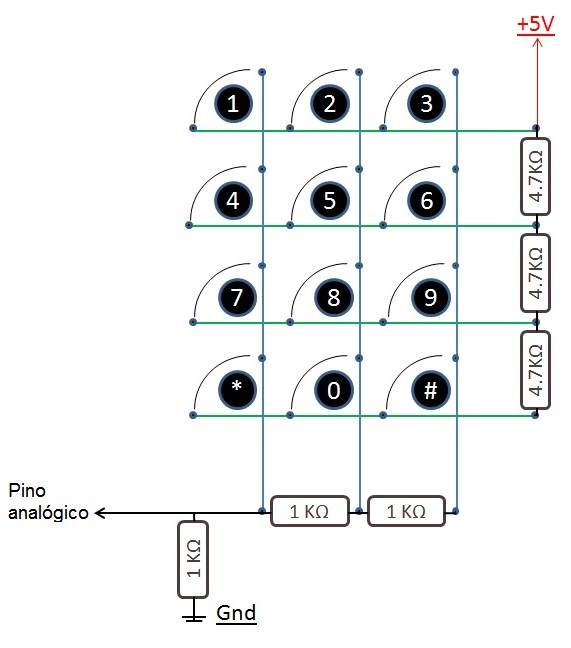
\includegraphics[scale=0.55]{figuras/cap4/onewirekeypad.jpg}\\
    Fonte: Adaptado de \cite{arduinocc_onewirekeypad}.
    \label{onewirekeypad}
    \end{center}
    \end{figure}
    
    
    \item Sensor Fingerprint
    
    O sensor Fingerprint faz a leitura de impressões digitais dos usuários. O processamento digital que envolve as operações de leitura e reconhecimento de impressões digitais, e o armazenamento das digitais são realizados no próprio sensor biométrico. Desta forma, são enviados comandos para que o sensor execute as ações desejadas. No total, o sensor possui apenas 4 pinos para conexão, 2 de alimentação e 2 de dados TTL serial (TX e RX). Portanto, o RX e TX do sensor devem ser conectados no TX e RX da MCU, respectivamente. Apesar de o Arduino Mega possuir somente 4 portas seriais, é possível conectar o sensor em outros pinos digitais que não dispõem de porta serial, através da criação de portas seriais virtuais. 
    
    \item MCU
    
    A MCU utilizada neste projeto é um microcontrolador Atmega 2560, responsável pelo processamento e manipulação dos dispositivos de entrada e saída no aparelho Setfinger.
    
    \item Controlador Ethernet
    
    O controlador ethernet provê a conexão do aparelho Setfinger à internet, assim estabelecendo a comunicação entre o aparelho Setfinger e o módulo servidor. O controlador ethernet é conectado a MCU através de comunicação SPI (\textit{Serial Peripheral Interface}), uma interface serial síncrona desenvolvido pela Motorola que permite a comunicação entre microcontroladores e periféricos, em comunicação de curta distância. Esse padrão pode ser utilizado em aplicações com cartões SD, \textit{displays} LCD, sensores, módulos RTC e até mesmo outros microcontroladores \cite{catsoulis2005designing, ganssle2007embedded, chattopadhyay2013embedded}. É importante ressaltar que no Arduino o controlador ethernet é conectado através do conjunto de pinos denominado \textit{ICSP}. Quando conectado ao Arduino Uno, os pinos 10, 11, 12 e 13 não podem ser utilizados. Se conectado ao Arduino Mega, os pinos 50, 51 e 52 não podem ser utilizados. Em ambos os casos os pinos citados não funcionarão para outras finalidades de I/O, pois são ocupados pela comunicação SPI (para mais detalhes, veja a documentação do Ethernet Shield \cite{ArduinoEthernetShield}).
    \nomenclature{I/O}{Entrada/saída (\textit{input/output})}
    
    \item Módulo Servidor
    
    O módulo servidor mantém as informações de controle de acesso dos usuários, estabelece a conexão com os clientes e disponibiliza o gerenciamentos de dados. Por se tratar de um módulo de \textit{software}, o servidor será abordado com mais detalhes na Seção~\ref{software}.
    
\end{itemize}
  
  Em relação as versões de \textit{hardware} apresentadas no Apêndice~\ref{hardware_1.0} e Apêndice~\ref{hardware_2.0}, a versão de \textit{hardware} proposta apresenta uma redução na quantidade de fios necessários para conectar o módulo de interface com o usuário ao módulo de \textit{hardware} interno (veja a Figura~\ref{circuit_setfinger_v3}). Essa redução de fios ocorre devido ao uso do circuito divisor de tensão \textit{one wire kaypad} e do módulo I2C em conjunto com o display LCD. A placa Setshield, mostrada na Figura~\ref{setshield_v3}, apresenta um resultado de PCB mais compacta em relação as versões 1.0 e 1.2. Além de tornar a placa Setshield mais compacta e reduzir a quantidade de fios, foi confeccionada uma carcaça menor e mais elegante para embutir os componentes de interface com o usuário (mostrada na Figura~\ref{setfinger_final}). Essa carcaça foi produzida em fibra de vidro com acabamento automotivo.
  
  O esquemático e o design da placa Setshield são produzidos no \textit{softwate} CadSoft Eagle 7.5.0 (veja o Apêndice~\ref{schematic_setshield} e Apêndice~\ref{board_setshield}).
  

\begin{figure}[!t]
  \begin{center}
  \caption{Circuito completo do \textit{hardware} Setfinger com todos os componentes conectados.}
  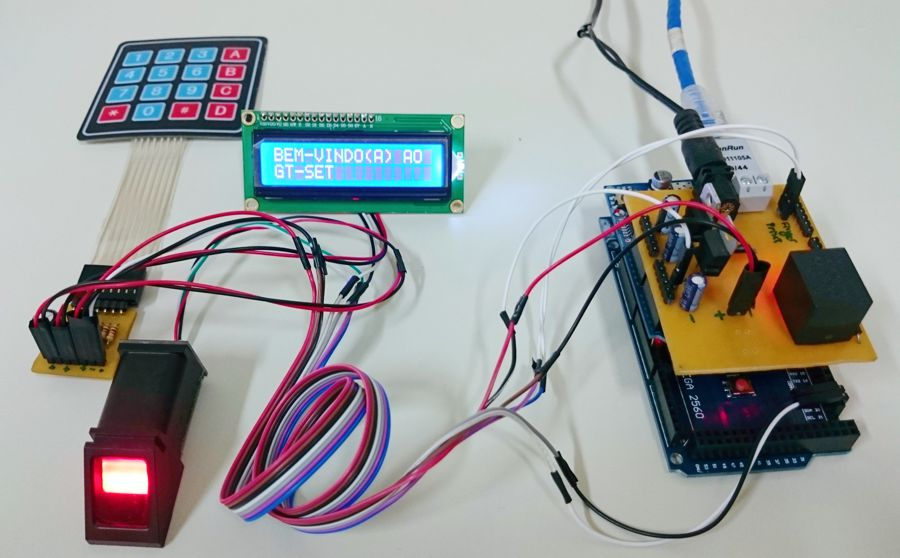
\includegraphics[scale=0.5]{figuras/cap4/circuit_setfinger_v3.jpg}\\
  Fonte: Elaborada pelo autor.
  \label{circuit_setfinger_v3}
  \end{center}
  \end{figure}
  
  
\begin{figure}[!t]
  \begin{center}
  \caption{Placa Setshield.}
  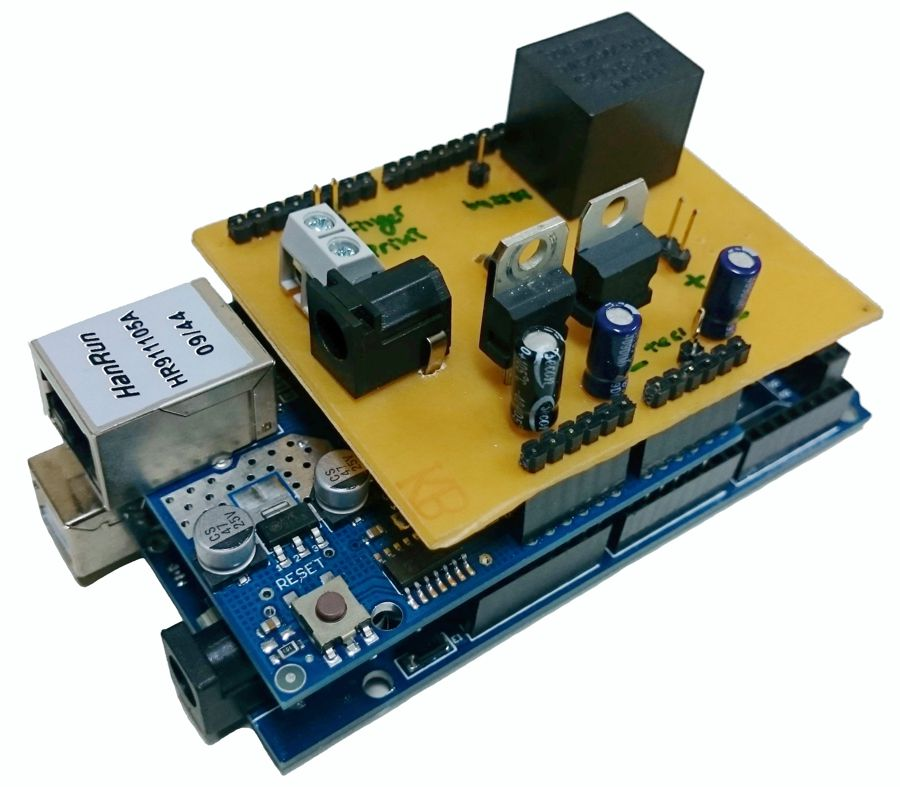
\includegraphics[scale=0.3]{figuras/cap4/setshield_v3.jpg}\\
  Fonte: Elaborada pelo autor.
  \label{setshield_v3}
  \end{center}
  \end{figure}
  

\begin{figure}[!t]
  \begin{center}
  \caption{\textit{Hardware} Setfinger -- módulo de interface com o usuário, composto por um display LCD, um leitor de impressões digitais e um teclado matricial do tipo membrana, embutidos em um gabinete de fibra de vidro. Este módulo deve ser instalado do lado externo do ambiente a ser controlado e próximo a porta}
  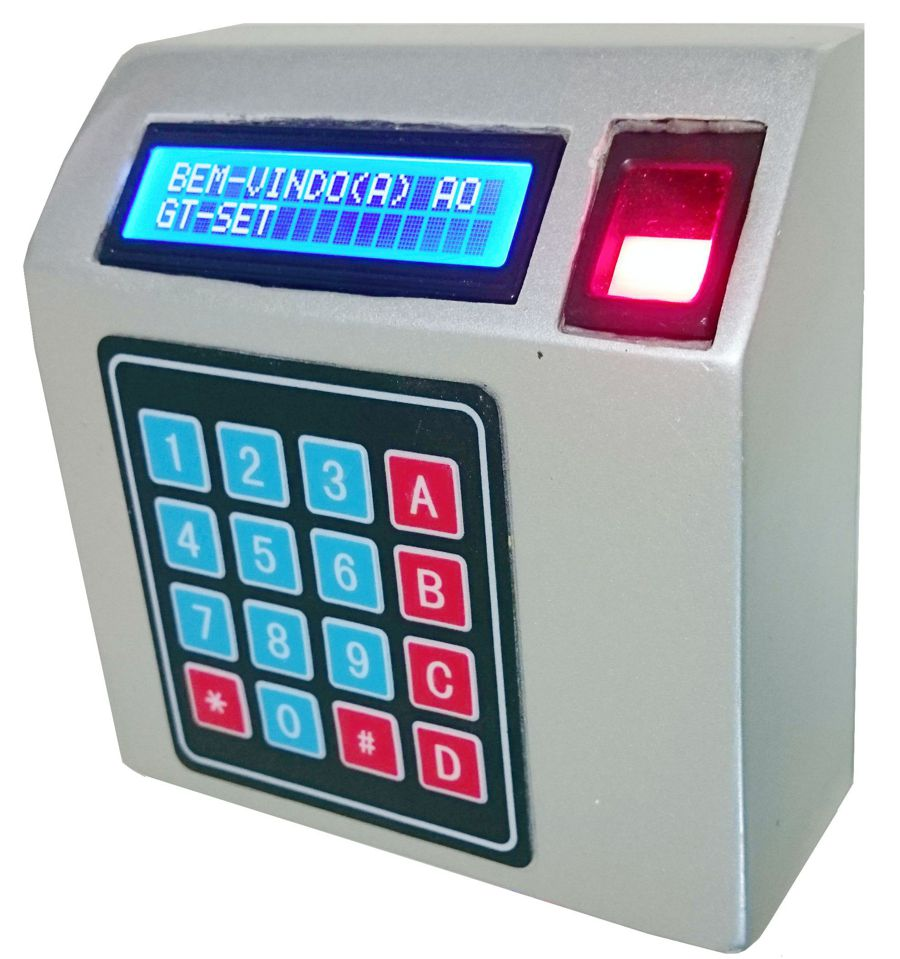
\includegraphics[scale=0.2]{figuras/cap4/setfinger_final.jpg}\\
  Fonte: Elaborada pelo autor.
  \label{setfinger_final}
  \end{center}
  \end{figure}





\section{\textit{Software} \label{software}}

Nesta seção serão abordados o banco de dados e os três módulos de \textit{software} que compõem o sistema Setfinger: cliente, servidor TCP e aplicação web. Entre o cliente e o servidor TCP há uma relação de dependência. Portanto, esses dois módulos serão apresentados em uma única seção para manter a organização do trabalho e simplificar a interpretação dos módulos  de \textit{software}. Por fim, será apresentada a aplicação de gerenciamento web.



\subsection{Cliente e servidor TCP}

O módulo de \textit{software} cliente é o \textit{software} embarcado na plataforma Arduino (MCU - Atmega 2560), escrito em linguagem C. Esse \textit{software} é responsável pela leitura da impressão digital do usuário, comunicação com o servidor TCP para verificar se tal usuário está cadastrado no banco de dados e qual seu nível de acesso, além de registrar o acesso desse usuário. O servidor TCP é uma aplicação do tipo server-side, desenvolvida com a plataforma node.js e escrita em linguagem javascript. Neste trabalho, essa aplicação possibilita a comunicação do cliente com o banco de dados que contém o cadastro e os registros de acesso dos usuários. Através dessa aplicação podem ser realizadas consultas e registros no banco de dados, de acordo com os comandos enviados pelo cliente. A lógica de funcionamento do aparelho Setfinger em conjunto com o servidor TCP pode ser melhor abstraída a partir do fluxograma mostrado na Figura~\ref{fluxograma_cliente-servidor}. Os principais blocos desse fluxograma são detalhados a seguir.

  
 \begin{figure}[!t]
 \begin{center}
  \caption{Fluxograma de funcionamento do aparelho Setfinger em conjunto com o servidor TCP - o fluxograma descreve as ações que envolvem o funcionamento do aparelho Setfinger em conjunto com o servidor TCP.}
  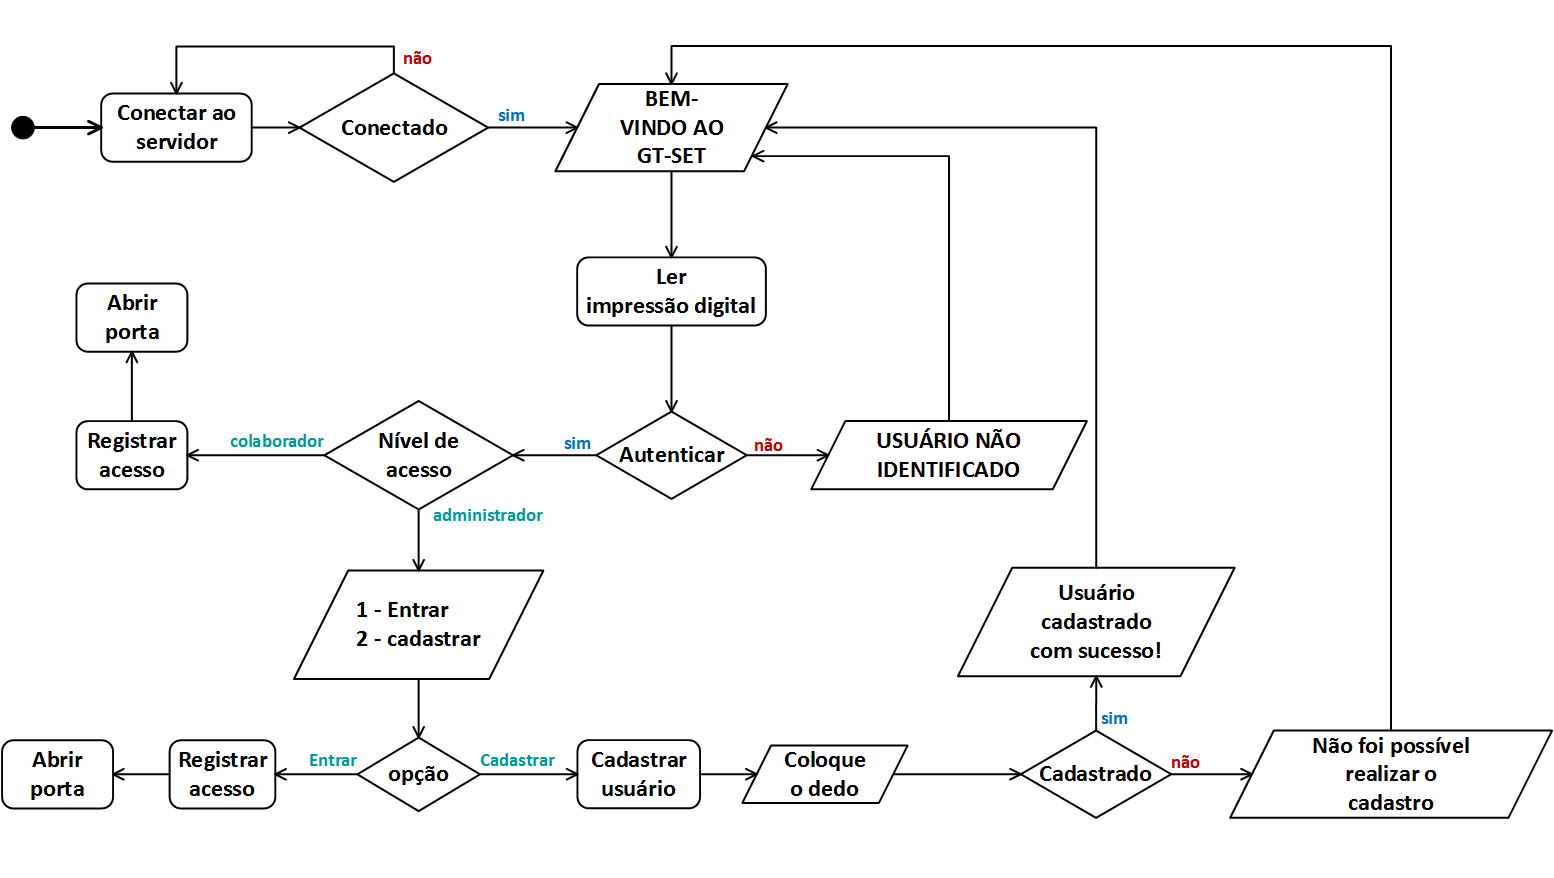
\includegraphics[scale=0.39]{figuras/cap4/fluxograma_cliente-servidor.png}\\
  Fonte: Elaborada pelo autor.
  \label{fluxograma_cliente-servidor}
  \end{center}
 \end{figure}
  
  \begin{itemize}
      \item Conectar ao servidor
      
      \begin{sloppypar}
      O cliente conecta-se ao servidor TCP através da execução da função \texttt{serverConnect()}, que faz parte do \textit{software} embarcado no Arduino (veja o Apêndice~\ref{apendice_conectar}). Essa função é responsável por estabelecer a conexão do cliente com o servidor TCP, através do método \texttt{client.connect(serverIP, serverPort)} nativo da biblioteca \textit{Ethernet.h}. Para estabelecer a conexão com o servidor TCP, o método \texttt{client.connect()} necessita receber o IP e a porta referentes ao servidor TCP. Essas configurações de IP e porta são definidas na declaração da biblioteca \texttt{Ethernet.h} (veja o Apêndice~\ref{apendice_ethernet}). Do lado do servidor é necessário utilizar o método \texttt{net.createServer()} para criar uma conexão do tipo TCP e atender as solicitações de conexão dos clientes (veja o Apêndice~\ref{apendice_createserver}).
      \end{sloppypar}
      
      Em qualquer ponto da execução do \textit{software} cliente, se a conexão for perdida por qualquer motivo, a execução volta para a conexão ao servidor.
      
      \item Ler impressão digital
      \begin{sloppypar}
      A função de leitura da impressão digital (\texttt{readFinger()}), implementada no \mbox{\textit{software}} cliente, realiza a captura da imagem da impressão digital e a comparação da impressão digital lida com as digitais cadastradas. As impressões digitais são armazenadas na memória \textit{flash} do sensor Fingerprint. A função que executa a leitura de impressões digitais no sensor Fingerprint é dividida em quatro eventos. \mbox{Esses} eventos são responsáveis por verificar se há um sensor conectado no sistema embarcado (\texttt{finger.verifyPassword()}), capturar a imagem da impressão digital (\texttt{finger.getImage()}), converter a imagem digital para um arquivo caracter (\texttt{finger.image2Tz()}) e buscar (\texttt{finger.fingerFastSearch()}) na memória do sensor, um arquivo carácter semelhante ao obtido na leitura da digital \cite{zfm-20}. Todos esses eventos (métodos) são nativos da biblioteca \texttt{Adafruit\_Fingerprint.h}. Desta forma, se a impressão digital lida for identificada, a função de leitura retornará um número do tipo inteiro que representa o ID associado a impressão digital identificada, caso contrário, a função deve retornar o valor $-1$.  
      \end{sloppypar}
      
      \item Autenticar
      
      Após a leitura da impressão digital, o ID retornado pela função \verb!readFinger()! é enviado para o servidor TCP no formato Notação de Objetos Javascript (\textit{Javascript Object Notation -- JSON})  \cite{bassett2015introduction, smith2015beginning}. O servidor TCP recebe o ID, consulta no banco de dados se há algum usuário com esse ID e responde ao cliente uma mensagem de erro, caso não haja nenhum usuário com tal ID, ou uma mensagem de confirmação com o nível de acesso do usuário autenticado. A digital do usuário deve estar cadastrada no sensor Fingerprint, porém a principal autenticação ocorre no servidor, pois o usuário pode estar cadastrado no sensor, mas se não estiver cadastrado no banco de dados, a sua autenticação não será confirmada. Isso facilita o gerenciamento online, tendo em vista que o gerenciamento remoto de usuários diretamente no sensor seria inviável.
      
      \nomenclature{JSON}{Notação de Objetos Javascript (\textit{Javascript Object Notation})}
      
      
      \item Nível de acesso
      
      Quando o ID informado no processo de autenticação pertencer a um usuário cadastrado no banco de dados, deve ser realizada uma consulta para verificar o nível de acesso desse usuário. Cada usuário possui um nível de acesso, o qual pode ser um colaborador (valor 0) ou um administrador (valor 1), de acordo com o diagrama de caso de uso mostrado na Figura~\ref{diagrama_autenticacao}. O nível de acesso de cada usuário será avaliado também na plataforma web.
      
      \begin{figure}[!t]
        \begin{center}
        \caption{Diagrama de caso de uso - autenticação do usuário no aparelho Setfinger.}
        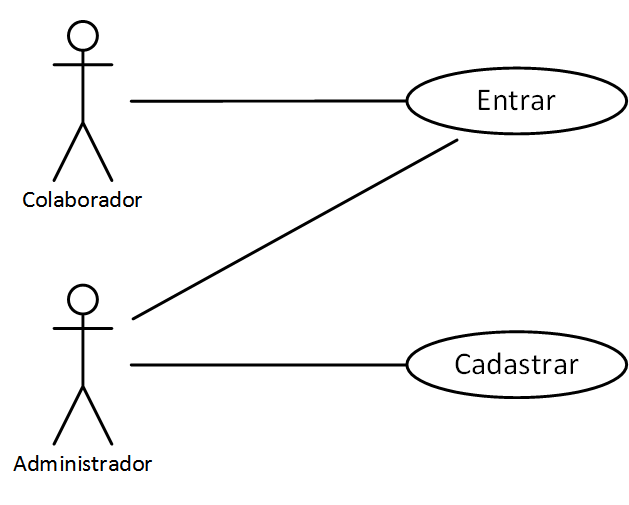
\includegraphics[scale=0.55]{figuras/cap4/diagrama_autenticacao.png}\\
        Fonte: Elaborada pelo autor.
        \label{diagrama_autenticacao}
        \end{center}
        \end{figure}
      
      \item Cadastrar usuário
      
      A operação de cadastro de usuário é dividida em duas etapas. A primeira etapa pode ser realizada somente através do aparelho Setfinger. Nessa etapa, é realizado o registro da impressão digital do usuário no sensor Setfinger. No ato do registro a impressão digital é gravada no sensor com um ID fornecido pelo servidor TCP, se a operação for realizada com sucesso o servidor TCP insere no banco de dados um novo usuário com o esse ID  e o nome ``NOVO USUÁRIO''. A memória flash do sensor Fingerprint tem um limite de $162$ impressões digitais \cite{zfm-20, zfm20ada}. Desta forma, quando a memória desse sensor estiver completamente ocupada, a reutilização de espaços de memória para registrar a impressão digital de novos usuário deve ser realizada somente quando o ID de uma impressão digital não pertencer a nenhum usuário cadastrado no banco de dados. Isto pode ocorrer quando um usuário for excluído do sistema. Portanto, o usuário pode estar cadastrado no sensor, mas se não estiver cadastrado no banco de dados, o espaço de memória ocupado pela sua digital poderá ser reutilizado. Logo, o controle de IDs é executado pelo servidor TCP e as informações referente as digitais disponíveis para o registro de novos usuários no sensor Fingerprint são mantidas no banco de dados, em uma tabela chamada \texttt{finger\_ids}.
      
      A segunda etapa de cadastro é possível somente após a ocorrência da primeira etapa. Nessa etapa, todos os usuários cadastrados como ``NOVO USUÁRIO'' devem permanecer na lista de Novos Usuário, até que o administrador do sistema atualize os dados de cada ``NOVO USUÁRIO'', através da plataforma web. 
      
      
      
      \item Registrar acesso
      
      Após a autenticação do usuário com nível de acesso ``colaborador'' ou após a escolha da opção ``Entrar'' por um usuário ``Administrador'', o aparelho Setfinger envia o ID do usuário para o servidor TCP, que insere no banco de dados o horário e a data de acesso desse usuário, em uma tabela chamada \verb!history!.
      
      \item Abrir porta
      
      A abertura da porta é a última operação a ser executada no processo de autenticação para acessar o ambiente controlado. No momento em que é autorizada a abertura da porta, um pino digital de saída ($5$ V) da MCU é setado em estado alto para acionar o relé associado ao fecho elétrico.
      
      \item Mensagens de display
      
      Durante a execução das operações previstas para o aparelho Setfinger, são exibidas mensagens em um display LCD para orientar o usuário na utilização do aparelho. A mensagem ``BEM-VINDO AO GT-SET'' é uma mensagem de boas vindas exibida sempre que o aparelho estiver no estado de leitura de impressão digital para autenticação, enquanto que as demais mensagens são exibidas de acordo com cada estado de operação do aparelho. Além disso, a mensagem de boas vindas ``BEM-VINDO AO GT-SET'' pode ser alterada diretamente no código do servidor TCP. Assim, no lugar de ``GT-SET'' pode ser colocado o nome do local em que o sistema Setfinger for instalado.
      
      
  \end{itemize}
  
  

\subsection{Plataforma web}

A plataforma web Setfinger possibilita o gerenciamento das informações mantidas no banco de dados. De acordo com o nível de acesso, essa plataforma classifica os usuários em duas categorias: os colaboradores e os administradores. Os colaboradores podem consultar somente seu próprio registro de acessos. Enquanto que os administradores do sistema podem atualizar o cadastro de usuários, consultar os acessos de usuários por data ou ID e gerar gráficos com base na frequência semanal ou mensal dos usuários. Na Figura~\ref{diagrama_autenticacao_web} são apresentados os casos de uso dos respectivos usuários. Esses casos de uso são discutidos nas Seções~\ref{sec:caso_uso:usuario} (colaboradores) e~\ref{sec:caso_uso:admin} (administrador).


\begin{figure}[!ht]
  \begin{center}
  \caption{Diagrama de caso de uso -- autenticação na plataforma web.}
  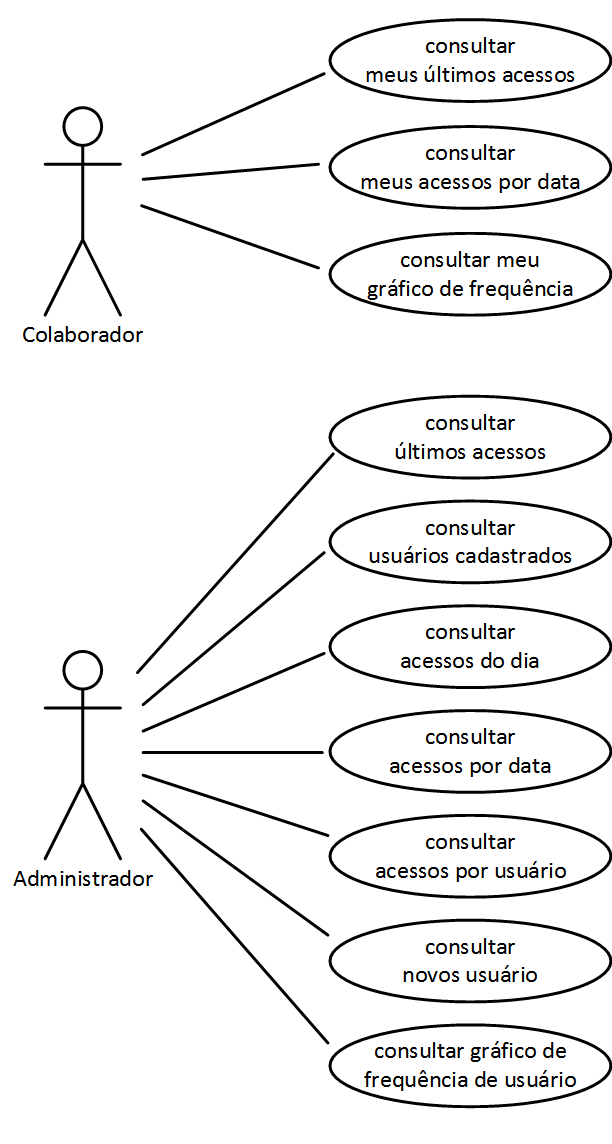
\includegraphics[scale=0.5]{figuras/cap4/diagrama_autenticacao_web.png}\\
  Fonte: Elaborada pelo autor.
  \label{diagrama_autenticacao_web}
  \end{center}
  \end{figure}
  
 Cada caso de uso apresentado no diagrama mostrado na Figura~\ref{diagrama_autenticacao_web} é uma página web. Essas páginas são divididas de acordo com as categorias de usuários. Portanto, as páginas de administrador são exclusivas ao acesso de administradores e as páginas de colaborador são exclusivas ao acesso de colaboradores. Além disso, essa plataforma possui uma tela de \textit{login} que antecede o acesso aos casos de uso. Esse \textit{login} é baseado em criptografia MD5 (\textit{Message-Digest algorithm 5}). Quanto a tecnologia, as páginas da plataforma proposta são responsivas, isto é, se redimensiona de acordo com o dispositivo que a executa (veja a Figura~\ref{setfinger_web}). Essa plataforma foi desenvolvida utilizando as linguagens HTML, CSS, PHP e Javascript e os \textit{frameworks} Bootstrap, Date picker bootstrap e Chart.js. A seguir, é apresentada uma descrição sucinta acerca de cada caso de uso.
 \nomenclature{MD5}{\textit{Message-Digest algorithm 5}}
  
\begin{figure}[!ht]
  \begin{center}
  \caption{Plataforma web Setfinger -- exemplo de uso em um dispositivo mobile.}
  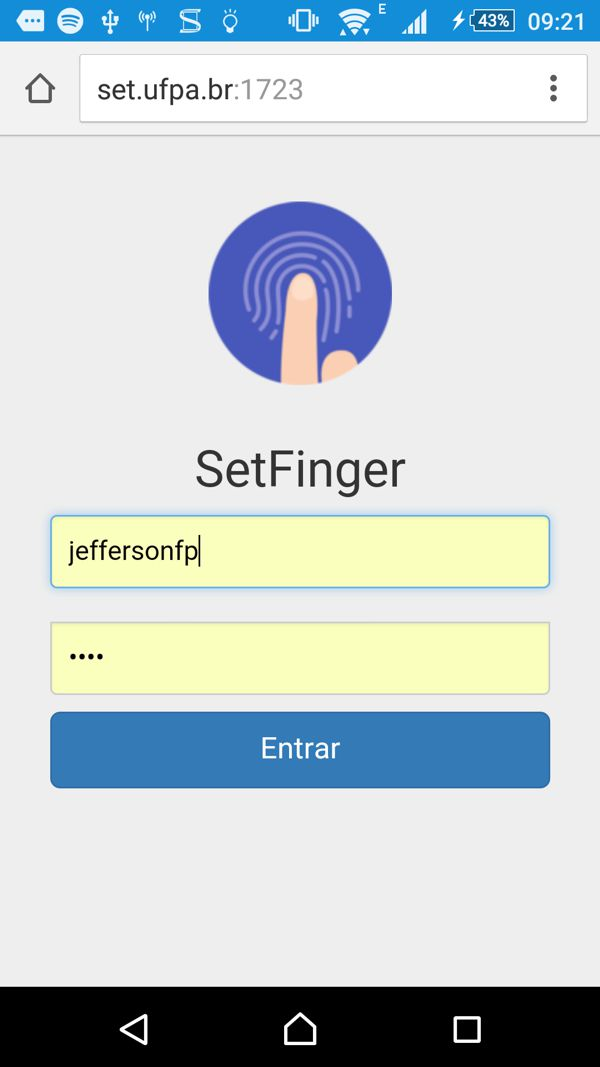
\includegraphics[scale=0.22]{figuras/cap4/setfinger_web.jpg}\\
  Fonte: Elaborada pelo autor.
  \label{setfinger_web}
  \end{center}
\end{figure}

  \subsubsection{Casos de uso dos colaboradores\label{sec:caso_uso:usuario}}
  \begin{itemize}
  
    \item Consultar últimos acessos
    
    Os últimos registros de acesso do colaborador são exibidos na página inicial da plataforma web, executada logo após o seu \textit{login}. Nessa página são exibidos os últimos 30 acessos registrados do colaborador.   
    
    \item Consultar meus acessos por data
    
    O colaborador pode consultar seus acessos por data. Desta forma, há um campo em que o usuário deve informar a data para a qual deseja consultar os seus registros de acessos.
    
    \item Consultar meu gráfico de frequência
  
    A partir dos registros de acesso do colaborador pode ser obtido o seu gráfico de frequência. Esse gráfico aponta a carga-horária mínima a ser cumprida e a carga-horária cumprida pelo colaborador dentro de um período que deve ser especificado no campo data (veja a Figura~\ref{web_frequencia_colaborador}).
  
    \begin{figure}[!ht]
    \begin{center}
    \caption{Plataforma web Setfinger - gráfico de frequência de usuário com nível de acesso \textit{colaborador}.}
     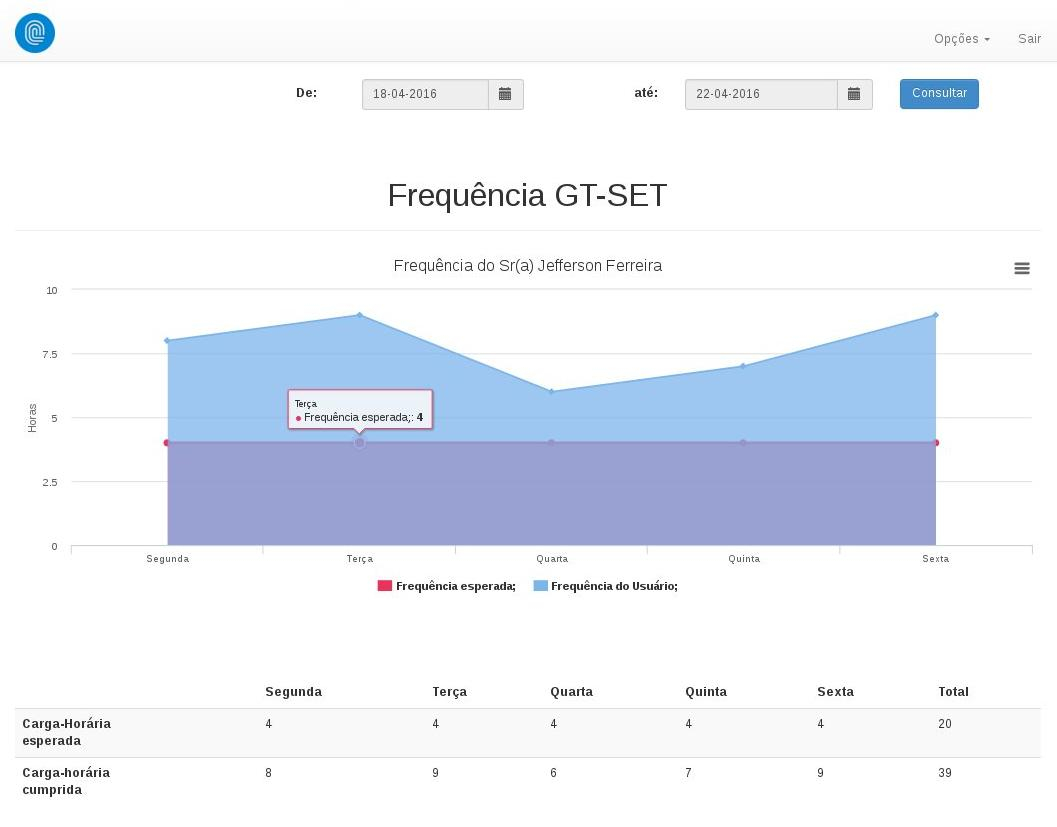
\includegraphics[scale=0.4]{figuras/cap4/web_frequencia_colaborador.jpg}\\
    Fonte: Elaborada pelo autor.
    \label{web_frequencia_colaborador}
    \end{center}
    \end{figure}
  
  
  
  \end{itemize}
  

  \subsubsection{Casos de uso dos administradores\label{sec:caso_uso:admin}}
  \begin{itemize}
  
    \item Consultar últimos acessos
    
    Na página inicial do administrador, executada após o seu \textit{login}, são exibidos os últimos 30 registros de acessos dos usuários cadastrados no sistema Setfinger.
    
    
    \item Consultar usuários cadastrados
    
    Usuários com nível de acesso \textit{administrador} podem consultar todos os usuários cadastrados no sistema. Nessa página são exibidos todos os usuários cadastrados no banco de dados, incluindo colaboradores e administradores, e seus dados.
    
    \item Consultar acessos do dia
    
    Os administradores podem consultar os registros de acessos ocorridos na data corrente.
    
    \item Consultar acessos por data
    
    Através dessa consulta são exibidos todos os registros de acessos ocorridos em uma data especificada pelo administrador.
    
    \item Consultar acessos por usuário
    
    Uma consulta pode ser realizada para verificar todos os registros de acessos de um usuário específico.
    
    \item Consultar novos usuários
    
    Todo usuário cadastrado no aparelho Setfinger é imediatamente cadastrado no banco de dados com o nome ``NOVO USUARIO'', permanecendo com o seu cadastro inativo até que seja realizada a atualização desse cadastro. Portanto, essa página exibe todos os usuários com atualização cadastral pendente.
    
    \item Consultar gráfico de frequência de usuário
  
    A partir dos registros de acessos de qualquer usuário, especificado ao sistema através do seu ID, pode ser gerado um gráfico de frequência. Esse gráfico aponta a carga-horária mínima a ser cumprida e a carga-horária efetiva cumprida pelo usuário dentro de um período, também especificado pelo administrador no campo data (veja a Figura~\ref{web_frequencia_admin}).
  
  
    \begin{figure}[!ht]
    \begin{center}
    \caption{Plataforma web Setfinger - gráfico de frequência de usuário com nível de acesso \textit{administrador}.}
     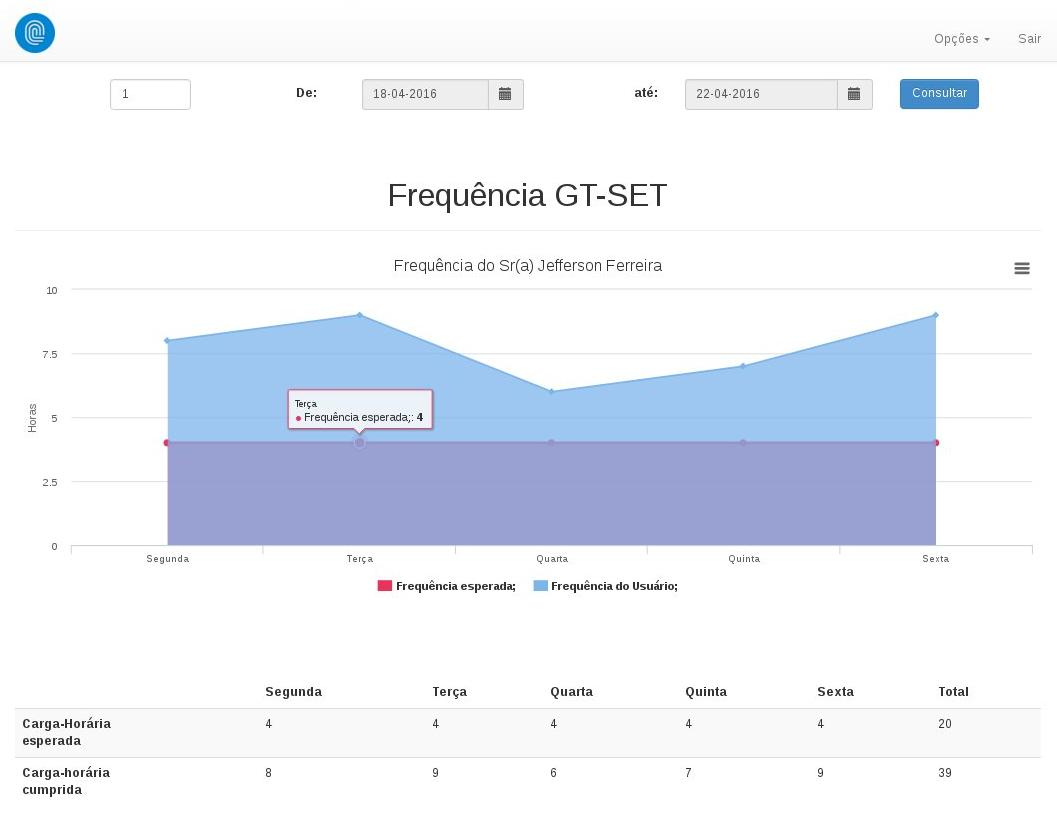
\includegraphics[scale=0.5]{figuras/cap4/web_frequencia_admin.jpg}\\
    Fonte: Elaborada pelo autor.
    \label{web_frequencia_admin}
    \end{center}
    \end{figure}
  
  
    
  \end{itemize}  
  
  
  
\subsection{Banco de dados}


A primeira etapa do projeto de um banco de dados é a construção de um modelo conceitual, através da modelagem conceitual. Um modelo conceitual é uma descrição abstrata do banco de dados, independente de implementação em um computador. O modelo conceitual registra os dados que devem aparecer no banco de dados, mas não registra como esses dados estão armazenados a nível de Sistema de Gerenciamento de Banco de Dados (\textit{Data Base Management System} -- DBMS). A técnica mais difundida de modelagem conceitual é a abordagem Modelo Entidade Relacionamento (\textit{Entity Relationship Model} -- ERM). Nessa técnica, um modelo conceitual é usualmente representado através de um diagrama, chamado Diagrama Entidade Relacionamento (\textit{Entity Relationship Diagram} -- ERD) \cite{heuser2009projeto}.

\nomenclature{DBMS}{Sistema de Gerenciamento de Banco de Dados (\textit{Data Base Management System})}
\nomenclature{ERM}{Modelo Entidade Relacionamento (\textit{Entity Relationship Model})}
\nomenclature{ERD}{(\textit{Entity Relationship Diagram})}


O uso de modelagem conceitual para projetar banco de dados pode auxiliar o DBMS a controlar a redundância de dados. A redundância de dados ocorre quando uma determinada informação está representada no sistema várias vezes, enquanto que a redundância controlada de dados acontece quando o \textit{software} tem conhecimento da múltipla representação da informação e garante a sincronia entre as diversas representações. Do ponto de vista do usuário externo ao sistema, tudo acontece como se existisse uma única representação da informação. Essa forma de redundância é utilizada para melhorar a performance global do sistema \cite{greenwald2007oracle, stephens2009sams}. Desta forma, são apresentados o modelo entidade-relacionamento e a modelagem do projeto de banco de dados do sistema Setfinger, nos diagramas mostrados na Figura~\ref{diagrama_DER} e Figura~\ref{diagrama_ER}, respectivamente.

\begin{sloppypar}
O diagrama mostrado na Figura~\ref{diagrama_ER} apresenta três tabelas: \texttt{finger\_ids}, \texttt{users} e \texttt{access}. 

A tabela \texttt{finger\_ids} é composta por 162 registros, cada registro contém um ID e o status de disponibilidade (\texttt{available}) desse ID, isto é, se o \texttt{available} de um ID for igual a $1$ significa que esse ID está disponível, caso seja igual a $0$ significa que está sendo utilizado por algum usuário. 

A tabela \texttt{users} contém os usuários cadastros. Portanto, cada registro contém os dados dos usuários, bem como, nome, \textit{login}, nível de acesso etc.

Por fim, a tabela \texttt{access} contém os registros de acesso dos usuários. Desta forma, cada registro contém a data e a hora de entrada do usuário no ambiente controlado.  



\end{sloppypar}

 \begin{figure}[!ht]
  \begin{center}
  \caption{Diagrama entidade-relacionamento - definição dos aspectos relacionais definidos para a modelagem do bando de dados do sistema Setfinger.}
  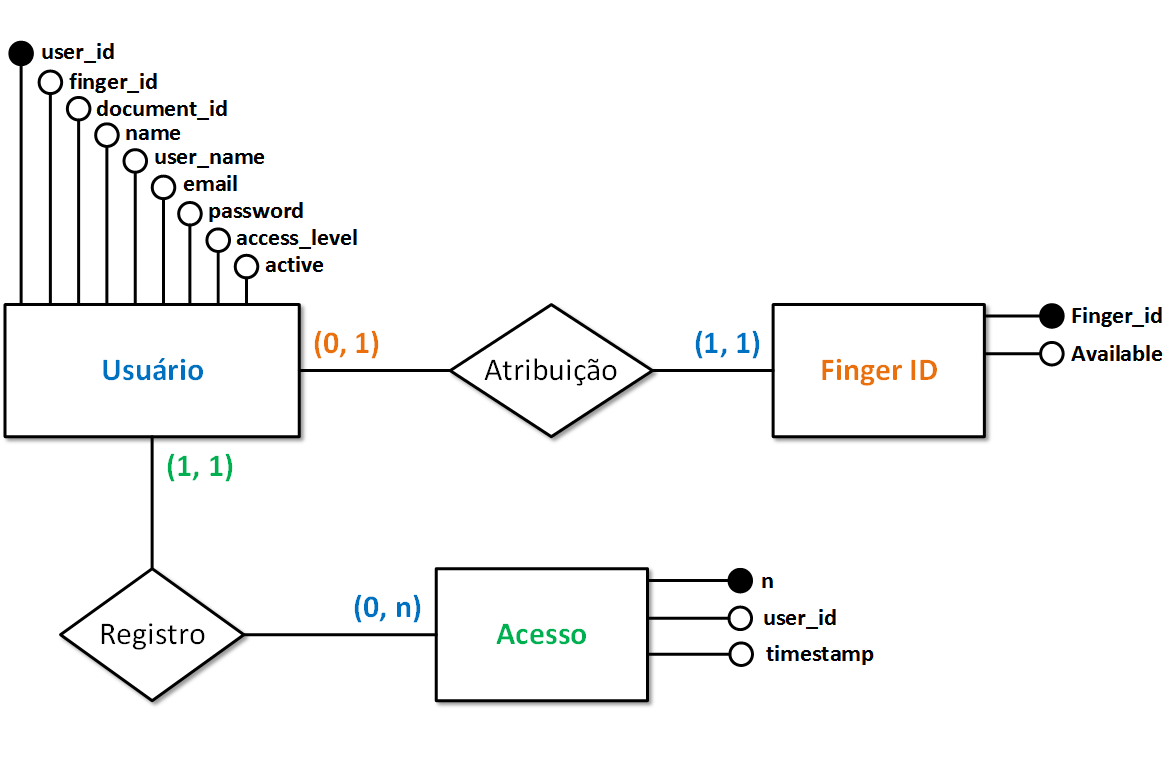
\includegraphics[scale=0.5]{figuras/cap4/diagrama_DER.png}\\
  Fonte: Elaborada pelo autor.
  \label{diagrama_DER}
  \end{center}
  \end{figure}
  
  
  
\begin{figure}[!ht]
  \begin{center}
  \caption{Diagrama de modelagem de banco de dados relacional - os relacionamentos entre as entidades do banco de dados do sistema Setfinger são definidos a partir do DBMS Phpmyadmin.}  
  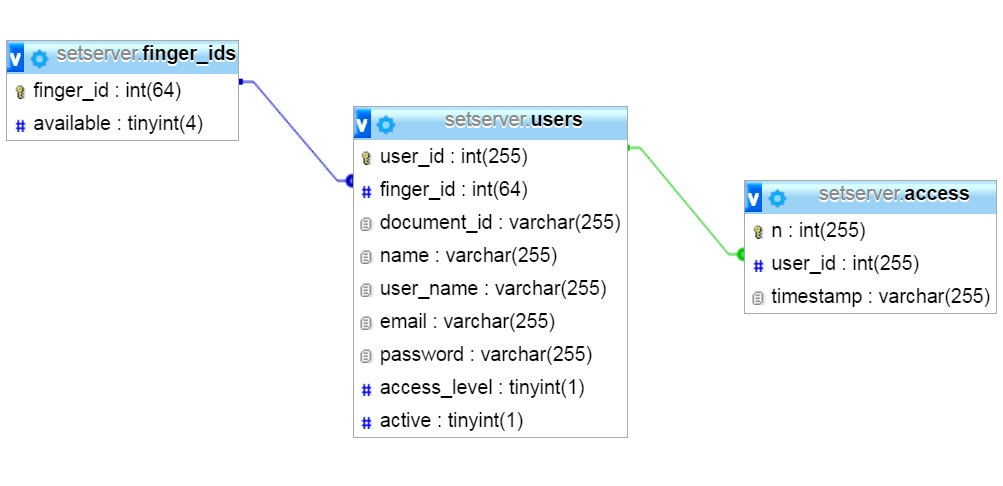
\includegraphics[scale=0.55]{figuras/cap4/diagrama_ER.jpg}\\
  Fonte: Elaborada pelo autor.
  \label{diagrama_ER}
  \end{center}
  \end{figure}
  

  

\section{Considerações}

Com relação ao desenvolvimento do módulo de \textit{hardware} houveram algumas dificuldades quanto a documentação de alguns dispositivos, como o sensor Fingerprint que possui \textit{datasheet} em inglês, porém pouco detalhada. Esse componente, assim como o display LCD, é de fabricação chinesa. Portanto, a documentação detalhada desses componentes estão disponíveis na língua Mandarin. O material empregado na confecção do aparelho Setfinger proposto na Seção~\ref{hardware_setfingerproposto}, custou R{\$} 404,55 (quatro centos e quatro reais e cinquenta e cinco centavos). A aquisição de grande parte desse material, tal como cabos com dimensão e número de conexões específicas, gabinetes para embutir o aparato eletrônico, CI's e outros componentes eletrônicos, foi difícil devido a baixa oferta desse tipo de produtos em Belém-Pa. Desta forma, houve a necessidade de encomenda de alguns componentes e adaptações utilizando materiais alternativos, para chegar o mais próximo possível do resultado desejado. Além disso, todos os diagramas e fluxogramas apresentados neste capítulo foram desenvolvidos no \textit{software} Microsoft Visio, com base na aplicação de Linguagem Unificada de Modelagem (\textit{Unified Modeling Language} -- UML) \cite{biafore2007visio, naiburg2001uml}. Exceto o diagrama de modelagem de banco de dados mostrado na Figura~\ref{diagrama_ER}, que foi elaborado do DBMS Phpmyadmin.

\nomenclature{UML}{Linguagem Unificada de Modelagem (\textit{Unified Modeling Language})}

Os códigos do sistema Setfinger estão disponíveis em \href{https://github.com/jeffersonfpalheta/setfinger_system}{\textit{github.com/jeffersonfpalheta}}.

